\documentclass[conference]{IEEEtran}
\IEEEoverridecommandlockouts

\usepackage[T1]{fontenc}
\usepackage[utf8]{inputenc}
\usepackage{cite}
\usepackage{amsmath,amssymb,amsfonts}
\usepackage{algorithm}
\usepackage{algpseudocode}
\usepackage{graphicx}
\usepackage{booktabs}
\usepackage{tabularx}
\usepackage{array}
\usepackage{xcolor}
\usepackage{tikz}
\usetikzlibrary{arrows.meta,positioning,calc}
\usepackage[hidelinks]{hyperref}
\usepackage{xurl}

\graphicspath{{figures/}}
\renewcommand{\tabularxcolumn}[1]{>{\raggedright\arraybackslash}m{#1}}
\newcolumntype{L}[1]{>{\raggedright\arraybackslash}p{#1}}
\newcommand{\ind}{\mathbb{1}}

\begin{document}

\title{Probabilistic Forecasting of Petroleum Imports and Supply-Shortfall Risk: Evidence from Kyrgyzstan and Other Landlocked Economies}

\author{\IEEEauthorblockN{Imanbek Mashrapov}
\IEEEauthorblockA{Informatics and Engineering Department\\
Ala-Too International University\\
Bishkek, Kyrgyzstan\\
Supervisor: Dr. Remudin Mekuria}}

\maketitle

\begin{abstract}
Landlocked economies buy refined fuel over a few overland routes and hold small stocks, so a supplier's decision can become a domestic shortage within weeks. Kyrgyzstan experienced this in mid-2026, when AI-95 gasoline ran out at Bishkek stations and the government banned fuel exports. Security-of-supply indices describe such dependence after the fact, and trade forecasting studies mostly predict annual values, so planners have no public, tested, forward-looking measure of how much fuel is likely to arrive.

This paper proposes a research framework to test whether monthly physical imports of refined petroleum, and the risk of a supply shortfall, can be forecast out of sample with calibrated uncertainty under real publication lags. It compares simple baselines, gradient boosting and small global neural models on a panel of landlocked economies, with Kyrgyzstan as the detailed case. The data stage is complete: 878 UN Comtrade responses were collected and validated, giving a main evaluation set of 22 series from 13 countries (3,021 observations) and a training pool of 44 series from 22 countries (5,549 observations). Kyrgyz gasoline agrees with the national energy balance within a mean absolute 3.7\% from 2018, and supplier data cover at least 90\% of import value in 99.4\% of series-months. Records from 2025 onward appear to be first-release figures, so the depth of the recent shock is uncertain. The data support a conditional decision to proceed. No forecasting model has yet been trained on the final datasets; all performance statements are hypotheses to be tested, and no new neural-network architecture is claimed.
\end{abstract}

\begin{IEEEkeywords}
petroleum imports, probabilistic forecasting, supply-shortfall risk, landlocked economies, global forecasting models, gradient boosting, conformal prediction, UN Comtrade, publication lag, Kyrgyzstan.
\end{IEEEkeywords}

\section{Introduction}

\subsection{Background and Motivation}
Most countries can receive fuel through several ports and suppliers. Landlocked economies cannot. Their fuel crosses at least one neighbouring country, usually by rail or road, and a small number of suppliers can account for almost all of it. A restriction imposed by one exporter can therefore reach domestic pumps quickly, particularly where storage is limited.

Kyrgyzstan is a clear example. It uses about 1.6--2 million tonnes of petroleum products a year by official and press estimates, and official statements put Russia's share of supply at about 93\% \cite{economist_stocks,kg24_exempt}. National import statistics exist, yet they are not designed to say how much fuel is likely to arrive next month, or how likely a shortfall is. The proposed study investigates whether public customs data can answer those two questions, and which modelling choices actually help.

\subsection{Refined Petroleum Supply in Landlocked Economies}
Refined products reach landlocked importers through customs-recorded purchases from a neighbouring refiner or a trading intermediary. The United Nations lists 32 landlocked developing countries \cite{ohrlls}; this study adds European landlocked economies because they report reliably and enlarge the training panel. The group is mixed: it contains low-income importers, transit markets, microstates and hydrocarbon producers. That diversity is both the reason a shared model might help and the main threat to it.

For a supply chain, the relevant quantity is not only the expected volume but also its reliability, because the import decision, stock policy and any emergency purchase all depend on the lower tail of the forecast.

\subsection{Export Restrictions and Supply-Shortfall Risk}
Russia restricted gasoline and diesel exports in September 2023 \cite{gta2023}, imposed a six-month gasoline ban from March 2024 \cite{enerdata2024}, and reinstated a ban for all exporters from October to December 2025 \cite{gta2025}. Supplies under intergovernmental agreements were formally exempt \cite{kg24_exempt}. Even so, when Russian refining output fell in 2026 the Kyrgyz market ran short: AI-95 ran out at Bishkek stations, fuel exports were banned, and stocks were reported at two to three weeks before recovering to about 1.5 months, against a government target of 2.5 months \cite{kwan2026,kunuz2026,economist_stocks}. A formal exemption did not guarantee physical supply.

Customs records show the event. In August 2026, Kyrgyz gasoline imports were 16.9 thousand tonnes (kt), about 39\% of the 2024--2025 monthly average, and Russia's share was 44\%. Two events do not validate a method, but they show that the target responds to documented supply stress.

\subsection{Role of Customs Data}
UN Comtrade \cite{comtrade} provides monthly records by reporter, six-digit Harmonized System (HS) code and partner, including net mass in kilograms, CIF value in US dollars and, in many cases, a first-release date. Mass and value are separate fields, so physical volume never has to be inferred from price. The limits are equally important: reporters publish late and irregularly, partner rows and aggregate rows can disagree, some masses are wrong, HS~2710.19 mixes several fuels, and records can be revised. These limits are treated here as part of the methodology rather than as incidental issues.

\subsection{Problem Statement}
The research problem is how far monthly physical imports of refined fuel in a landlocked economy can be forecast, together with a calibrated statement of uncertainty and shortfall risk, using only information available on the forecast date. The problem is wider than point forecasting. It comprises (i) a validated physical target, (ii) point and quantile forecasts, (iii) shortfall probability, (iv) calibration under publication lag and revision, and (v) a usable monitoring tool.

\subsection{Research Gap}
Trade forecasting has moved towards graph and neural models \cite{zhao2026,sellami2024,ma2024}, security-of-supply research has developed concentration indices \cite{cohen2011,lecoq2009,ang2015}, and customs-based early warning has reached product level for a maritime economy \cite{kwon2026}. Existing studies have addressed these components largely as separate problems, which leaves an opportunity to test them together for monthly physical fuel flows in landlocked economies (Section~\ref{sec:gap}).

\subsection{Research Objective}
The primary objective is to determine whether monthly physical imports of refined petroleum and supply-shortfall risk in landlocked economies can be forecast with useful, calibrated accuracy, and to establish under what conditions global Deep Learning improves on gradient boosting and simple baselines. Specific objectives are to (1) build an audited, reproducible dataset; (2) define a shortfall target that separates supply stress from weak demand; (3) compare models under rolling-origin evaluation that respects publication lag; (4) measure by ablation the value of pooling, supplier structure and shock information; (5) calibrate forecasts and evaluate shortfall warnings against concentration screening; and (6) deliver a working risk monitor.

\subsection{Research Questions}
The research questions are listed below and mapped to methodology and evaluation in Table~\ref{tab:alignment}.

\begin{description}
\item[RQ1] Does cross-country training improve Kyrgyz forecasts over local models and seasonal naive?
\item[RQ2] Do global neural models outperform gradient boosting, in normal and shock periods?
\item[RQ3] Do supplier structure and shock information add predictive value beyond a series' own history?
\item[RQ4] Can calibrated forecasts warn of shortfalls better than concentration screening?
\end{description}

\subsection{Research Hypotheses}
The following are working hypotheses, fixed before modelling, to be tested at the 5\% level with Holm correction \cite{holm1979}. A finding that a hypothesis is not supported is an acceptable and informative outcome.

\begin{description}
\item[H1] Global models reduce Kyrgyz MASE by at least 5\% relative to the best local model at $h=3$.
\item[H2] Neural models do not beat LightGBM overall, but do beat it in shock windows.
\item[H3] Adding supplier and shock information reduces pinball loss by at least 3\% for high-dependence series.
\item[H4] Forecast-based shortfall probability gives higher PR-AUC, and better recall at a fixed alert budget, than ranking by the Herfindahl--Hirschman index (HHI).
\end{description}

\subsection{Research Contributions}
Three levels of contribution are distinguished. The scientific contribution is a tested benchmark of global Deep Learning against gradient boosting for monthly physical fuel imports in landlocked economies, including an out-of-sample test of whether concentration screening works where one supplier dominates. The methodological contribution is a transparent route from customs records to a validated physical target, with explicit treatment of publication lag and data vintage. The applied contribution is a public-data risk monitor. The study does not claim the invention of a new neural-network architecture.

\begin{table*}[t]
\centering
\caption{Alignment of research questions, hypotheses, methodology, evaluation and the expected type of result.}
\label{tab:alignment}
\small
\begin{tabularx}{\textwidth}{@{}c c >{\hsize=1.05\hsize}X >{\hsize=0.95\hsize}X X@{}}
\toprule
RQ & H & Methodological component & Evaluation & Expected type of result\\
\midrule
1 & 1 & Local vs.\ global models; strict-importer panel (Sec.~\ref{sec:global}) & MASE at $h=3$, HLN test & Value of pooling, possibly negative\\
2 & 2 & LightGBM, XGBoost, GRU, TCN, N-BEATS, compact TFT (Sec.~\ref{sec:baselines}, \ref{sec:neural}) & Errors stratified by normal and shock windows & Paired comparison with effect sizes\\
3 & 3 & Supplier and shock feature ablation (Sec.~\ref{sec:ablation}) & Pinball loss, high-dependence series & Marginal value of each information source\\
4 & 4 & Conformal calibration and exceedance probability (Sec.~\ref{sec:uq}, \ref{sec:shortfall}) & PR-AUC, recall at alert budget, calibration & Comparison with HHI screening\\
\bottomrule
\end{tabularx}
\end{table*}

\subsection{Scope and Delimitations}
The study focuses on monthly imports of a gasoline proxy (HS~271011/12) and of distillates with blends (HS~271019 + 271020) from January 2015 to August 2026. Liquefied petroleum gas is descriptive only. Crude oil and the 2710 heading total are excluded as targets. Separate diesel, jet-fuel and fuel-oil targets are not possible at six digits. Customs records measure imports, not consumption, and the models are not intended to predict political decisions.

\subsection{Thesis Structure}
Section~\ref{sec:lit} reviews the literature and derives the research gap. Section~\ref{sec:method} describes the methodology, and Section~\ref{sec:data} reports the completed data validation. Section~\ref{sec:arch} presents the system architecture, Section~\ref{sec:exp} the experimental design and Section~\ref{sec:expected} the expected results as a discussion framework. Section~\ref{sec:limits} covers limitations, ethics and risks, and Section~\ref{sec:conclusion} concludes. The final report will follow the faculty's five sections: Problems, Aim/Objectives, Methods and Material, Outcomes and Application. Because this is a proposal, the experimental and discussion sections specify planned evaluation; only Section~\ref{sec:data} and the labelled pilot report executed work.

\section{Literature Review}\label{sec:lit}

\subsection{Customs Data for Supply Analysis}
Kwon and Jeong \cite{kwon2026} are the closest precedent. Using Korean imports of 5,925 HS six-digit products from 2010 to 2025 in a walk-forward design, they report top-5\% watchlist precision of about 1.7 times the base rate, with 31\% of onsets caught, and find that concentration ranks below the base rate as a short-run signal. The setting differs from this study in three ways: Korea is maritime, the target is all goods, and the output is a ranking, not a calibrated volume.

\subsection{Security of Supply and Import Dependence}
Security-of-supply research measures dependence through diversification and risk indices \cite{cohen2011,lecoq2009,ang2015}. Such indices are useful descriptions, but they look backward and are rarely tested as predictors. Work on the resilience of the global oil trade network uses simulation to show that diversification and flexible rewiring help \cite{chen2025}; it does not forecast out of sample.

\subsection{Forecasting Fuel and Trade Flows}
Country studies of petroleum imports are often explanatory or use one model on value data \cite{pradhan2023,santi2023}. Neural studies of trade report strong results, but some choices limit what can be learned from them. Khajoui et al. \cite{khajoui2024}, for example, convert annual data to 200 seasonal values and claim 99\% accuracy; interpolating a target in this way inflates the sample and is avoided here.

\subsection{Statistical and Tree-Based Approaches}
Exponential smoothing and SARIMA are natural local references. Tree ensembles, such as random forests \cite{breiman2001}, XGBoost \cite{chen2016} and LightGBM \cite{ke2017}, are robust on tabular features. Gradient boosting dominated the M5 accuracy competition \cite{makridakis2022}, and trees still lead on many tabular problems \cite{grinsztajn2022}, so they are treated here as the main rival rather than as a formality.

\subsection{Recurrent Networks for Short Series}
Long short-term memory \cite{hochreiter1997} and gated recurrent units \cite{cho2014} remain standard sequence models \cite{hewamalage2021}. In Turkish agri-food trade, SARIMA was best for regular exports and GRU for volatile imports \cite{abedi2025}, which supports testing Deep Learning by regime, not assuming it.

\subsection{Global Forecasting Models}
Models trained across related series often outperform local ones, and this is a statement about data structure rather than architecture \cite{montero2021,semenoglou2021,hewamalage2022}. It is the only reason Deep Learning is feasible here: about 130 Kyrgyz points cannot train a network, while a pooled panel may support a small one. The benefit is not automatic if the series are unrelated.

\subsection{Transformers and Long-Horizon Models}
The Temporal Fusion Transformer provides quantile output and variable selection \cite{lim2021}. However, a linear model has challenged long-horizon Transformers on far larger datasets \cite{zeng2023}. With only 140 monthly steps per series, this study excludes large Transformers on evidence and tests only a compact TFT.

\subsection{Graph Models of Trade}
Graph attention \cite{velickovic2018} and related models have been applied to trade networks \cite{zhao2026,sellami2024}, usually at annual or aggregate scale and in value terms. About 20 country nodes do not provide a defensible graph-learning problem, so supplier links enter here as features, and a graph layer is only a single optional ablation arm.

\subsection{Probabilistic Forecasting}
DeepAR showed the value of probabilistic global models \cite{salinas2020}, proper scoring rules give the evaluation standard \cite{gneiting2007}, and conformalized quantile regression offers a way to correct interval coverage \cite{romano2019}. Modern networks can be poorly calibrated \cite{guo2017}, so calibration must be evaluated rather than assumed.

\subsection{Structural Change}
Li et al. showed that training windows crossing structural change can damage gasoline demand forecasts \cite{li2022}. The period 2022--2026 offers a direct test for imports, where sanctions, export bans and shifting suppliers all occur within the evaluation window.

\subsection{Evaluation Standards}
Scaled errors allow comparison across series \cite{hyndman2006}; rolling-origin testing replaces random splits \cite{tashman2000}; cross-validation needs care for autoregressive problems \cite{bergmeir2018}; and pairwise tests such as Diebold--Mariano with the Harvey correction are standard but have low power on short samples \cite{diebold1995,harvey1997}.

\subsection{Critical Review of Existing Research}
Table~\ref{tab:related} compares the principal works. Three observations follow. First, reported gains come from different datasets, frequencies and splits, so rankings of architectures across papers are not reliable. Second, most trade studies predict value, whereas a planner needs tonnes. Third, the studies closest to the problem do not provide calibrated volumes. A critical caveat is that many papers here were assessed at abstract level, and each must be read in full before the final thesis.

\begin{table*}[t]
\centering
\caption{Comparison of principal related studies and their relevance to the proposed research.}
\label{tab:related}
\small
\begin{tabularx}{\textwidth}{@{}L{2.2cm} L{3.1cm} X X X@{}}
\toprule
Study & Problem & Data & Method & Limitation / relevance\\
\midrule
Kwon and Jeong \cite{kwon2026} & Import disruption early warning & Korea, 5,925 HS6 products, monthly, 2010--2025 & Gradient boosting, logistic, walk-forward & Maritime; all goods; ranking, no neural models\\
Zhao et al. \cite{zhao2026} & Global trade network prediction & 187 countries, 1995--2021 & Graph attention, temporal convolution, GBDT & Aggregate scale; no refined products\\
Sellami et al. \cite{sellami2024} & Bilateral trade prediction & Comtrade, annual, 5,000+ product groups & GCN and GAT vs.\ random forest & Annual; value not mass\\
Abedi \cite{abedi2025} & SARIMA, LSTM, GRU compared & T\"urkiye agri-food, monthly & Comparative time series & One country; not energy\\
Pradhan et al. \cite{pradhan2023} & Petroleum import trend & Nepal (landlocked), 1987--2018 & Trend analysis & No forecast comparison\\
Santi et al. \cite{santi2023} & Oil and gas import value & Indonesia & SARIMA & Value; one model\\
Chen et al. \cite{chen2025} & Oil trade network resilience & Global trade data & Risk-propagation simulation & No out-of-sample forecast\\
Cohen et al. \cite{cohen2011} & Security of supply & Diversification measures & Index & Backward looking\\
\bottomrule
\end{tabularx}
\end{table*}

\subsection{Identified Research Gap}\label{sec:gap}
A new country alone is not a gap. The gap appears when the requirements of the problem are compared with what the closest streams provide. (i) Trade forecasting predicts annual or value flows at large scale. (ii) Security-of-supply research measures dependence after the fact. (iii) Customs early warning, which is closest, targets a coastal economy across all goods and ranks products. No study was found that tests, for landlocked economies, whether monthly physical refined-fuel imports and shortfalls can be forecast out of sample with calibrated uncertainty under real publication lags, or whether pooling across such countries and adding supplier information helps. This is a finding of the stated search, which was run through OpenAlex, Crossref, Semantic Scholar and arXiv, not proof that no such study exists. The study does not assume the integrated approach is superior; that is the empirical question.

\section{Research Methodology}\label{sec:method}

\subsection{Research Design}
The study follows a quantitative, comparative, data-driven design. It is organised as a sequence of controlled comparisons, each answering one research question by changing one component (model class, information source or output type) while holding the data, validation protocol and metrics fixed.

\subsection{Overall Research Framework}
The framework (Fig.~\ref{fig:workflow}) runs from raw public data to a monitoring tool. The first three stages are complete; modelling begins only after the rules are reviewed and frozen.

\begin{figure*}[t]
\centering
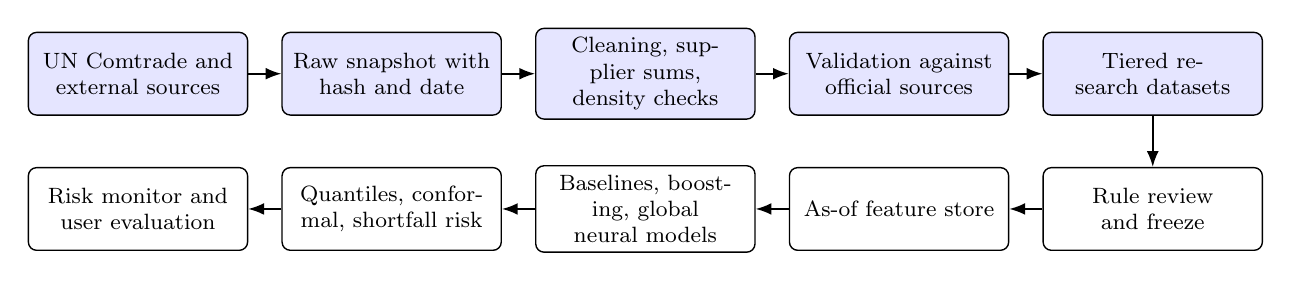
\begin{tikzpicture}[
  box/.style={draw, rounded corners=3pt, align=center, font=\footnotesize, minimum height=1.05cm, text width=2.55cm, line width=0.5pt},
  done/.style={box, fill=blue!10},
  plan/.style={box, fill=white},
  arrow/.style={-{Latex[length=2mm]}, line width=0.6pt},
  node distance=0.42cm]
\node[done] (a) {UN Comtrade and external sources};
\node[done, right=of a] (b) {Raw snapshot with hash and date};
\node[done, right=of b] (c) {Cleaning, supplier sums, density checks};
\node[done, right=of c] (d) {Validation against official sources};
\node[done, right=of d] (e) {Tiered research datasets};
\node[plan, below=0.65cm of e] (f) {Rule review and freeze};
\node[plan, left=of f] (g) {As-of feature store};
\node[plan, left=of g] (h) {Baselines, boosting, global neural models};
\node[plan, left=of h] (i) {Quantiles, conformal, shortfall risk};
\node[plan, left=of i] (j) {Risk monitor and user evaluation};
\foreach \x/\y in {a/b,b/c,c/d,d/e,e/f,f/g,g/h,h/i,i/j} \draw[arrow] (\x) -- (\y);
\end{tikzpicture}
\caption{Overall research workflow. Shaded stages are complete; unshaded stages are planned.}
\label{fig:workflow}
\end{figure*}

\subsection{Data Sources}
The primary source is UN Comtrade \cite{comtrade}, queried by API with credentials held only in the environment. Validation uses the Kyrgyz Fuel and Energy Balance \cite{nsc_balance} and tables and operational reports of the National Statistical Committee (NSC). Exogenous data are Brent \cite{eia_brent}, global and Russia geopolitical risk \cite{caldara2022}, monthly exchange rates and consumer prices, and annual World Bank indicators \cite{wdi}. Table~\ref{tab:sources} summarises them.

\begin{table}[t]
\centering
\caption{Data sources used in the project.}
\label{tab:sources}
\small
\begin{tabularx}{\columnwidth}{@{}L{2.45cm} L{1.15cm} X@{}}
\toprule
Source & Freq. & Use\\
\midrule
UN Comtrade & Monthly & Target, suppliers, exports, release dates\\
Russia as reporter & Monthly & Mirror check, ends Dec.\ 2021\\
NSC energy balance & Annual & Mass, dependency, stock cover, to 2024\\
NSC commodity tables & Annual & Value check, to 2025\\
NSC monthly reports & Monthly & All goods; first and latest vintage\\
Brent, WTI & Daily & External condition\\
Global, Russia GPR & Monthly & External condition\\
Exchange rate, CPI & Monthly & 27 of 28 countries\\
GDP, population & Annual & Scale only; never interpolated\\
\bottomrule
\end{tabularx}
\end{table}

\subsection{Comtrade Data Structure}
Each bilateral record is a tuple $(i, k, j, f, t, m, v)$ with reporter $i$, HS code $k$, partner $j$, flow $f$, month $t$, net mass $m$ in kilograms and customs value $v$ in US dollars. Grouped records are then produced at reporter--product--month level. Table~\ref{tab:vars} lists the planned variable groups.

\begin{table}[t]
\centering
\caption{Planned variable groups.}
\label{tab:vars}
\small
\begin{tabularx}{\columnwidth}{@{}L{1.25cm} X L{1.75cm}@{}}
\toprule
Group & Variables & Leakage control\\
\midrule
Temporal & Lags 1--12, rolling mean and dispersion, seasonal lag, month encoding & Released data only\\
Price & Lagged unit value, Brent level and change & Lag to release date\\
Risk & Global and Russia GPR, documented restriction in force & Announced by origin\\
Supplier & HHI over trailing 12 months, Russia share, top-supplier share, neighbour exposure & Trailing windows\\
Macro & Exchange rate, CPI & Lag to release date\\
Static & Country identity, product, importer type & Verified, fixed\\
\bottomrule
\end{tabularx}
\end{table}

\subsection{Product Identification}
HS six-digit codes define the products. The gasoline proxy merges 271011 (HS 2007) with 271012 (from HS 2012). HS~271019 holds diesel, kerosene, jet fuel, fuel oil and lubricants together, and blended diesel moves to 271020, so the distillate target is the sum 271019 + 271020, which makes reporters comparable. The label is ``distillates'', never ``diesel''.

\subsection{Data Cleaning}
Net weight is used when positive. Other quantity fields are accepted only when the unit is literally kilograms. Where a volume appears on the same row, the implied density must be physically possible (gasoline 0.68--0.80~kg/L, LPG 0.48--0.62, others 0.60--1.05). Unit value is compared with a plausible band and with its centred 13-month median after Brent deflation: too low means mass is overstated, so mass is removed and the original kept; too high only raises a flag. Outliers beyond four robust deviations on log mass are flagged and kept, because shocks are the object of study. Unit conversion is limited to kilograms to tonnes.

\subsection{Missing Data and Reporting Gaps}
Missing values are never replaced with zero and target values are never interpolated. Each month carries a status: observed, mass rejected by check, value without mass, no record in a published month, reporting interruption, or outside the reporting span. A missing month is left out of the loss and not scored. Short gaps in neural inputs may be filled for inputs only, with a mask feature. Annual values are not spread across months.

\subsection{Monthly Series Construction}
Monthly totals are rebuilt from partner rows, because the ``World'' row can be zero or too low while partner rows contain trade. Algorithm~\ref{alg:series} outlines the procedure.

\begin{algorithm}[t]
\caption{Monthly series construction (conceptual)}
\label{alg:series}
\begin{algorithmic}[1]
\For{each reporter $i$, product $k$, month $t$}
  \State Remove duplicates on the natural key; keep latest retrieval
  \State Resolve mass; apply the density rule to each row
  \State Sum partner rows, or use the World row with a label
  \State Compare partner sum with World row
  \State Test unit value; reject implausible mass, keep original
  \State Assign a data status; retain the first-release date
\EndFor
\State Compute supplier measures on partner rows
\State Assign tiers using frozen coverage rules
\end{algorithmic}
\end{algorithm}

\subsection{Supplier Concentration and Import Dependency}
With $s_{ijt}$ the share of partner $j$ in the import mass of series $i$ in month $t$,
\begin{equation}
\mathrm{HHI}_{it}=\sum_{j} s_{ijt}^{2}.
\label{eq:hhi}
\end{equation}
Because one thin month can dominate \eqref{eq:hhi}, the study pools mass over a trailing year, $\mathrm{HHI}^{12}_{it}$, with at least six observed months required. Concentration says how few suppliers a country uses. Dependency says how much of its use is imported, and is computed annually for Kyrgyzstan only:
\begin{equation}
\mathrm{DEP}_{y}=\frac{\mathrm{Imports}_{y}-\mathrm{Exports}_{y}}{\mathrm{DomesticUse}_{y}}.
\label{eq:dep}
\end{equation}
Values above one mean that imports also went into stocks.

\subsection{Temporal Feature Engineering}
Volumes are modelled in log tonnes. Features include lags 1--12, rolling means and dispersion over observed months with a count of months available, a seasonal lag, and month encodings. Neural inputs are normalised per window, so countries of different size can share weights.

\subsection{External Indicators}
Brent, geopolitical risk, exchange rates and CPI are candidates only. Exploratory correlations are weak (Section~\ref{sec:external}), so each must earn its place in ablation. Exploratory correlation is not treated as causation.

\subsection{Shock and Policy Variables}
A hand-coded calendar will record documented export restrictions with source and date. A restriction may be used only once announced by the forecast origin. Sparse events create strong imbalance, and they are not assumed sufficient for a stand-alone classifier.

\subsection{Dataset Construction}
A sample is defined at forecast origin $\tau$ for series $i$: a history window, static features, external indicators, supplier features and targets for horizon $h\in\{1,3,6\}$ plus the next-three-month total. The information set contains only what had been released by the origin:
\begin{equation}
\mathcal{F}_{i,\tau}=\{x_{it}: r_{it}\leq\tau\},
\label{eq:asof}
\end{equation}
where $r_{it}$ is the release date of observation $t$. Each forecast is
\begin{equation}
\hat{y}^{(q)}_{i,\tau+h}=f_{\theta}\!\left(\mathcal{F}_{i,\tau}, s_{i}, h, q\right),
\label{eq:forecast}
\end{equation}
with $s_i$ static features and $q$ a quantile level.

\subsection{Training, Validation and Test Strategy}\label{sec:split}
Evaluation uses an expanding rolling origin \cite{tashman2000}, with origins running monthly from January 2023 to the last available month. Random splitting is not used, because neighbouring months share shocks and would produce optimistic estimates. Tuning uses data before each test block, normalisation is fitted on the input window or training period, and hyperparameters and feature sets freeze before a final block that is run once. Leave-one-country-out training tests transfer. Leakage sources to be controlled are release dates, later-revised values, same-month unit values, look-ahead cleaning fields, and restrictions not yet announced.

\begin{table}[t]
\centering
\caption{Planned model progression. Complexity increases downward; the purpose is to test whether added complexity yields measurable improvement.}
\label{tab:models}
\small
\begin{tabularx}{\columnwidth}{@{}L{2.9cm} L{1.3cm} X@{}}
\toprule
Model & Scope & Role\\
\midrule
Naive, seasonal naive, 12-month mean & Local & Lower bound\\
ETS, SARIMA & Local & Reference (H1)\\
Random forest & Global & Tree baseline\\
LightGBM, XGBoost & Local, global & Main rival (H2)\\
GRU, TCN, N-BEATS & Global & Neural candidates (H2)\\
Compact TFT & Global & Quantiles, variable selection\\
Graph attention layer & Global & Optional ablation arm\\
\bottomrule
\end{tabularx}
\end{table}

\subsection{Baseline Models}\label{sec:baselines}
Baselines progress in complexity (Table~\ref{tab:models}) so that the benefit of each component can be measured. The seasonal naive and 12-month mean are essential, because a model that cannot beat them has no value. Gradient boosting uses quantile objectives on lag-feature tables \cite{ke2017,chen2016}.

\subsection{Global Neural Models}\label{sec:neural}
The GRU \cite{cho2014} updates a hidden state as
\begin{align}
z_t&=\sigma(W_z[h_{t-1},x_t]),\quad r_t=\sigma(W_r[h_{t-1},x_t]),\nonumber\\
\tilde{h}_t&=\tanh(W[r_t\odot h_{t-1},x_t]),\nonumber\\
h_t&=(1-z_t)\odot h_{t-1}+z_t\odot\tilde{h}_t.
\label{eq:gru}
\end{align}
The TCN \cite{bai2018} uses dilated causal convolutions,
\begin{equation}
F(t)=\sum_{l=0}^{L-1} w_l\, x_{t-d\,l},
\label{eq:tcn}
\end{equation}
with filter length $L$ and dilation $d$, so that the receptive field grows without recurrence. N-BEATS \cite{oreshkin2019} stacks fully connected blocks that subtract a backcast and add a forecast. Capacity is deliberately small: 16--64 hidden units, a country embedding of size 8, and dropout. The compact TFT \cite{lim2021} has a hidden size below 32 and is dropped if validation does not support it. These are hypotheses to test, not assumptions of superiority.

\subsection{Global Pooling}\label{sec:global}
A global model shares $\theta$ in \eqref{eq:forecast} across all series. Pooling may help through shared dynamics, even though Section~\ref{sec:eda} finds little shared movement. A local version of each model and a strict-importer panel test this directly.

\subsection{Supplier Graph Features}
Shared-supplier exposure is computed as a trailing feature: the weighted recent change in a neighbour's imports from the same supplier. An optional single graph attention layer \cite{velickovic2018} is compared with these hand-built features. It is not a primary model.

\subsection{Probabilistic Forecasting}\label{sec:uq}
Quantile models minimise the pinball loss
\begin{equation}
\rho_q(u)=u\left(q-\ind[u<0]\right),\quad u=y-\hat{y}^{(q)}.
\label{eq:pinball}
\end{equation}
Conformalized quantile regression \cite{romano2019} then widens or narrows a pair of quantiles using scores from a calibration window:
\begin{equation}
E_n=\max\!\left\{\hat{y}^{(\ell)}_n-y_n,\ y_n-\hat{y}^{(u)}_n\right\},
\label{eq:cqr}
\end{equation}
with the corrected interval $[\hat{y}^{(\ell)}-\hat{Q},\ \hat{y}^{(u)}+\hat{Q}]$, where $\hat{Q}$ is the empirical $(1-\alpha)$ quantile of $E$. Its coverage guarantee assumes exchangeability, which time series may violate, so coverage is measured and not assumed. The pilot gave nominal 80\% intervals with only 62--75\% Kyrgyz coverage, which justifies this step.

\subsection{Shortfall Target and Risk}\label{sec:shortfall}
Let $Q_{it}$ be the trailing three-month mass and $B_{it}$ the mean of the same three calendar months in the previous three years. A shortfall month satisfies
\begin{equation}
S_{it}=\ind\!\left[\,Q_{it}/B_{it}<0.75\,\right].
\label{eq:shortfall}
\end{equation}
A supply-side shortfall additionally has a positive standardised change in unit value, which separates supply stress from weak demand. Thresholds of 0.70 and 0.80 are sensitivity checks. Risk is derived from the forecast distribution rather than an unverifiable label:
\begin{equation}
\hat{p}_{i,\tau+h}=\Pr\!\left(Q_{i,\tau+h}/B_{i,\tau+h}<0.75\mid\mathcal{F}_{i,\tau}\right).
\label{eq:risk}
\end{equation}
Labels are a proxy, are not verified disruptions, and will be checked against the sourced event list before use.

\subsection{Explainability}
Tree SHAP \cite{lundberg2017} will be applied to LightGBM, and variable selection to the TFT if retained. Findings are checked with domain logic, and error is analysed by country, product, season, supplier dependence and importer type. No feature-importance values are reported in this proposal.

\subsection{Evaluation Metrics}
Table~\ref{tab:metrics} defines the metrics. MASE is primary. With $n$ test months and in-sample seasonal differences of period $m$,
\begin{equation}
\mathrm{MASE}=\frac{\frac{1}{n}\sum_{t}|y_t-\hat{y}_t|}{\frac{1}{T-m}\sum_{t=m+1}^{T}|y_t-y_{t-m}|},
\label{eq:mase}
\end{equation}
\begin{equation}
\mathrm{WAPE}=\frac{\sum_{t}|y_t-\hat{y}_t|}{\sum_{t}|y_t|},\
\mathrm{Brier}=\frac{1}{n}\sum_{t}(\hat{p}_t-S_t)^2.
\label{eq:wape}
\end{equation}
Mean absolute percentage error is not used, since near-zero months make it unstable, and $R^2$ is not used for model selection.

\begin{table}[t]
\centering
\caption{Evaluation metrics and why they are used.}
\label{tab:metrics}
\small
\begin{tabularx}{\columnwidth}{@{}L{1.3cm} L{2.5cm} X@{}}
\toprule
Task & Metric & Why it is relevant\\
\midrule
Point & MASE, WAPE, RMSE, MAE, sMAPE & Comparable across countries \cite{hyndman2006}\\
Quantile & Pinball loss, CRPS approximation & Proper scoring \cite{gneiting2007}\\
Interval & 80\% and 95\% coverage, width & Coverage versus sharpness\\
Shortfall & PR-AUC, ROC-AUC, Brier, calibration, recall at alert budget, lead time & PR-AUC suits rare events \cite{saito2015,brier1950}\\
Compare & HLN test, Holm correction, block bootstrap & Low power, so effect sizes are also reported\\
\bottomrule
\end{tabularx}
\end{table}

\section{Data Validation and Exploratory Results}\label{sec:data}
This section reports executed work on snapshot 2026-11-02 (dataset version 1.0.0). It is descriptive, and no forecasting model was fitted.

\subsection{Coverage and Country Tiers}
Candidates were screened into three tiers (Fig.~\ref{fig:coverage}). Tier~1 requires at least 120 observed months, 85\% coverage of the 140-month window, no gap above six months, data reaching June 2025 or later, at least 84 supplier months, a median of at least 100~t, exports below half of imports, and no classification flag. Tier~2 needs at least 84 observed and supplier months. The result is 22 Tier~1 series in 13 countries with 3,021 observations for evaluation, and 44 Tier~1 and Tier~2 series in 22 countries with 5,549 observations for training. Kyrgyzstan is the only Central Asian country in Tier~1; Kazakhstan and Uzbekistan are Tier~2, and Tajikistan and Turkmenistan have no monthly data. Twelve of 22 gasoline series reach June 2026, and eight of the 22 panel countries have a median release lag of at least 200 days.

\begin{figure}[t]
\centering
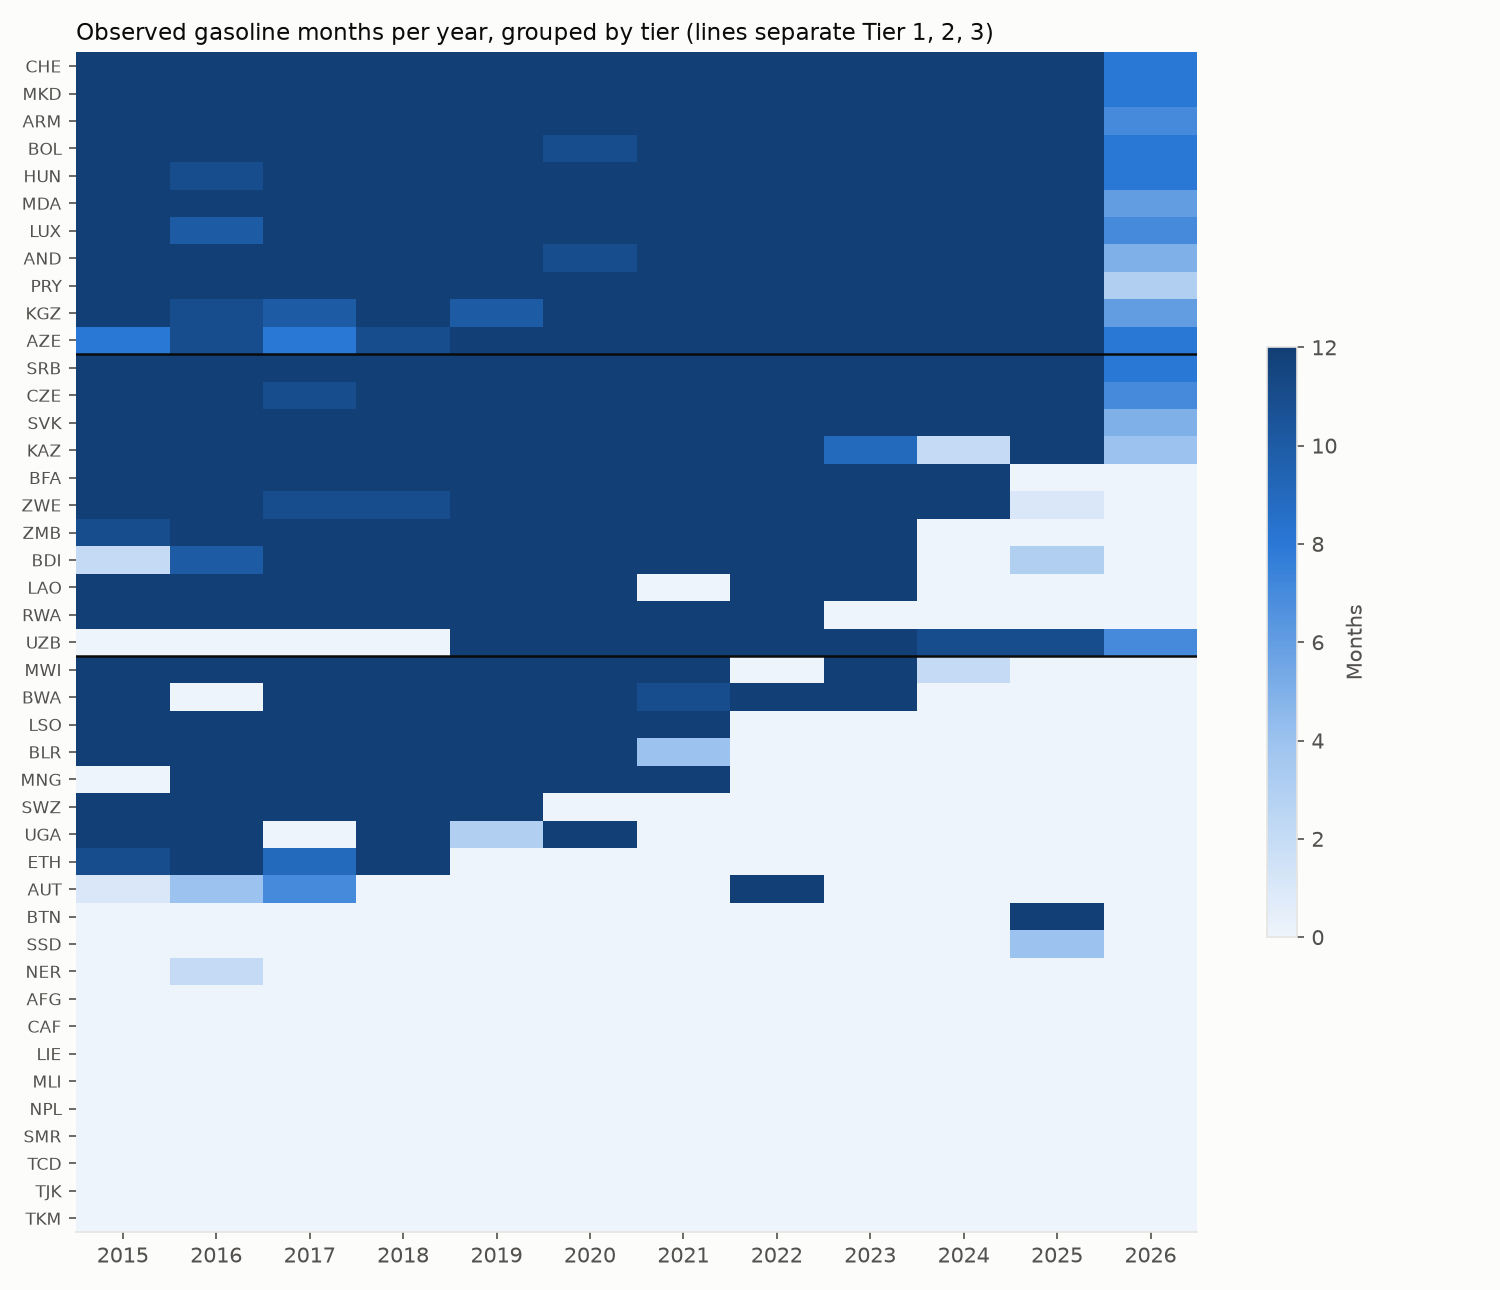
\includegraphics[width=\columnwidth]{fig09_coverage_heatmap}
\caption{Observed gasoline months per year by reporter. Lines separate Tiers 1, 2 and 3.}
\label{fig:coverage}
\end{figure}

\subsection{Kyrgyz Target}
Comtrade publishes 136 of the 140 Kyrgyz months; 133 are usable for each product. Sep.--Oct.\ 2019 and Jun.--Jul.\ 2026 are absent, and three months per product were rejected by checks. Fig.~\ref{fig:monthly} shows both series. Monthly gasoline swings widely around a stable level, while distillates rise from 2024. The October--November 2017 gasoline records imply a density of about 1.42~kg/L; they were rejected and held apart as a labelled volume estimate.

\begin{figure*}[t]
\centering
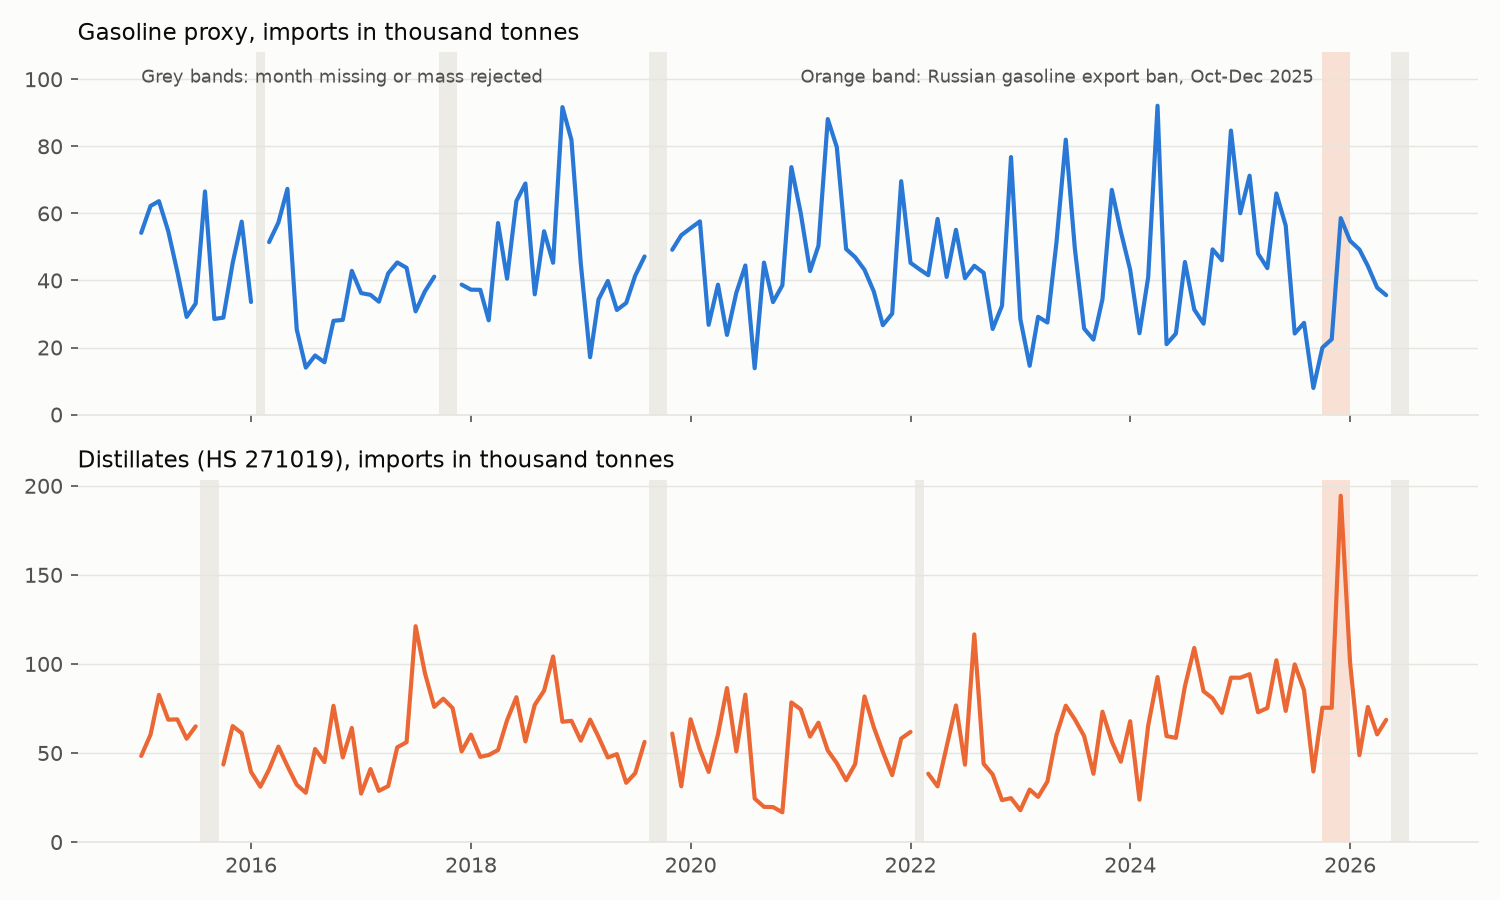
\includegraphics[width=0.86\textwidth]{fig01_kyrgyz_monthly_imports}
\caption{Kyrgyz monthly imports, January 2015 to August 2026, in thousand tonnes. Grey bands mark months missing or rejected; nothing is interpolated.}
\label{fig:monthly}
\end{figure*}

\subsection{Validation Against Official Sources}
Table~\ref{tab:validation} and Fig.~\ref{fig:reconcile} summarise the checks. Gasoline mass agrees with the balance within a mean absolute 3.7\% from 2018, and exports match it closely (2024: 77.6 and 76.4~kt). Russia's exports to Kyrgyzstan are about three times recorded imports in 2016--2017, and exceed the national balance as well (1,023 and 533~kt in 2016), so simple Kyrgyz under-recording does not explain the difference. The cause is unknown, so results will be reported with and without 2015--2017.

\begin{table}[t]
\centering
\caption{Kyrgyz validation results.}
\label{tab:validation}
\small
\begin{tabularx}{\columnwidth}{@{}X L{3.4cm}@{}}
\toprule
Check & Result\\
\midrule
Gasoline mass vs.\ balance & 3.7\% mean abs.\ diff.\ from 2018\\
Gasoline value vs.\ NSC table & Within 5\% in 2022--2024\\
2025 gasoline value vs.\ NSC & Ratio 0.78\\
Gasoline exports vs.\ balance & 2024: 77.6 and 76.4 kt\\
Partner rows vs.\ World & No month over 5\% in value\\
Russian mirror, 2018 and 2021 & 0.93--1.02\\
Russian mirror, 2016--2017 & 0.33--0.37\\
\bottomrule
\end{tabularx}
\end{table}

\begin{figure}[t]
\centering
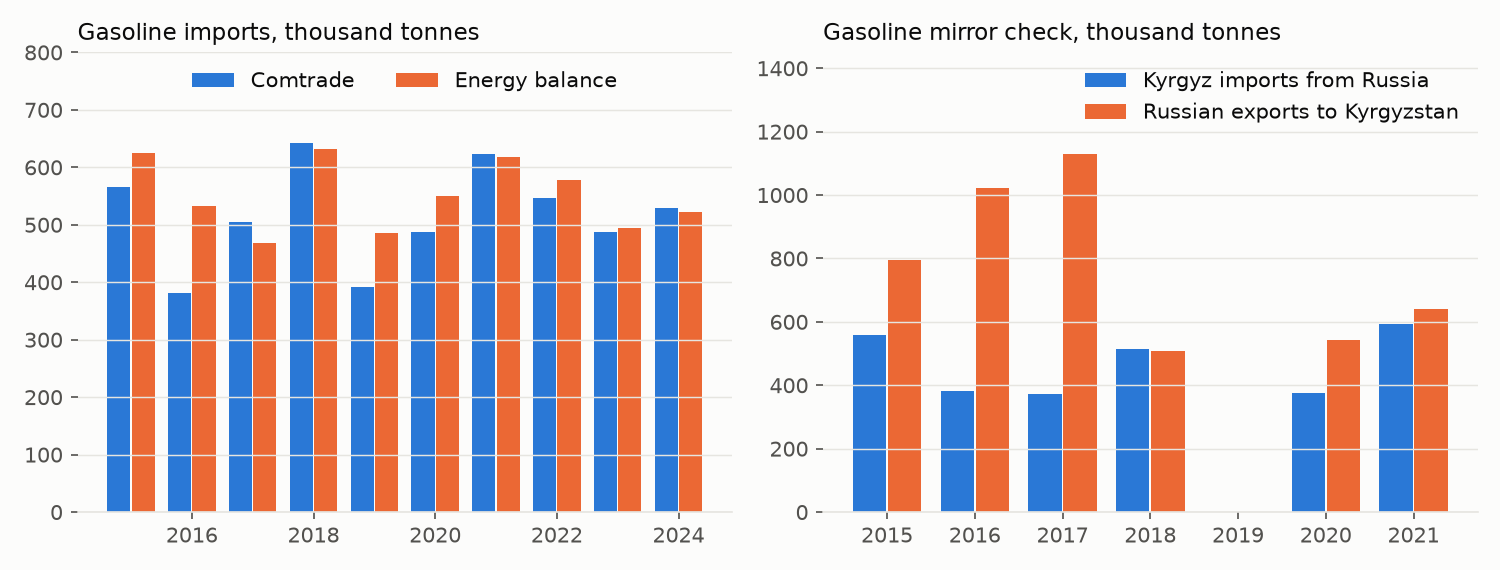
\includegraphics[width=\columnwidth]{fig11_kyrgyz_reconciliation}
\caption{Gasoline against the energy balance (left) and the Russian mirror (right). 2017 Comtrade includes the labelled volume estimate.}
\label{fig:reconcile}
\end{figure}

\subsection{First-Release Vintage}
For all goods, each month from 2025 was compared with the first and latest figure in monthly NSC reports (Fig.~\ref{fig:vintage}). Of the 16 months with a revised national figure, 12 match the first release within 1\%, none matches the latest, and the latest national figure runs about 9\% higher at the median. The 2025 gasoline value is 0.78 of the official figure, against 0.95--1.00 in 2022--2024. Part of the late-2025 fall in gasoline may therefore be under-recording. The all-goods evidence cannot say how much applies to fuel, which is why the 2025 balance and repeated snapshots matter.

\begin{figure}[t]
\centering
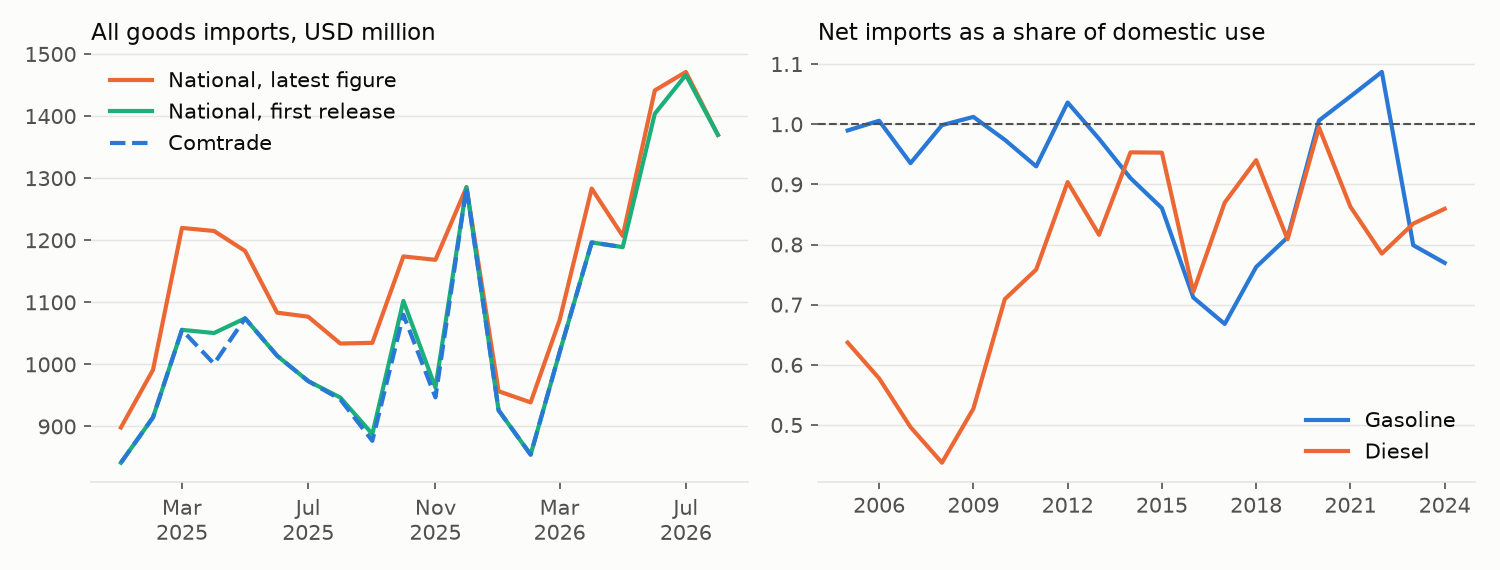
\includegraphics[width=\columnwidth]{fig12_kyrgyz_vintage_and_dependency}
\caption{First and latest all-goods figures against Comtrade (left), and annual net import dependency (right).}
\label{fig:vintage}
\end{figure}

\subsection{Exploratory Patterns}\label{sec:eda}
Kyrgyz gasoline varies by month (Kruskal--Wallis $p<0.001$), highest in December (1.36 of the annual mean) and lowest in September (0.66), while HS~271019 has no clear pattern ($p=0.42$), as Fig.~\ref{fig:season} shows. So the widely assumed seasonal farm demand for distillates must be tested. Across the panel, STL \cite{cleveland1990} gives a median seasonal strength of 0.22. PELT \cite{killick2012} places level shifts in gasoline at July 2025 and in distillates at April 2024 (Fig.~\ref{fig:breaks}); the first coincides with both Russian restrictions and first-release months, so its size is uncertain. Co-movement is weak: the median pairwise correlation of year-on-year gasoline changes is 0.04, and 0.01 for Kyrgyzstan.

\begin{figure}[t]
\centering
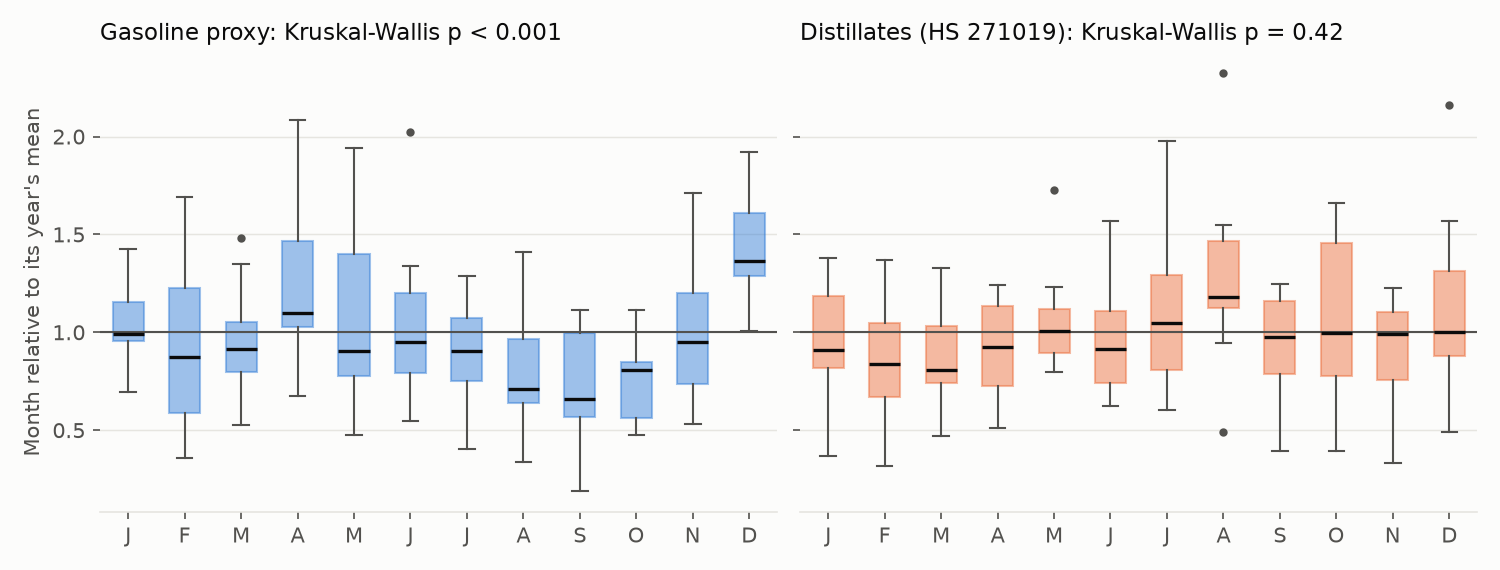
\includegraphics[width=\columnwidth]{fig03_kyrgyz_seasonality}
\caption{Month relative to its year's mean for Kyrgyz imports.}
\label{fig:season}
\end{figure}

\begin{figure}[t]
\centering
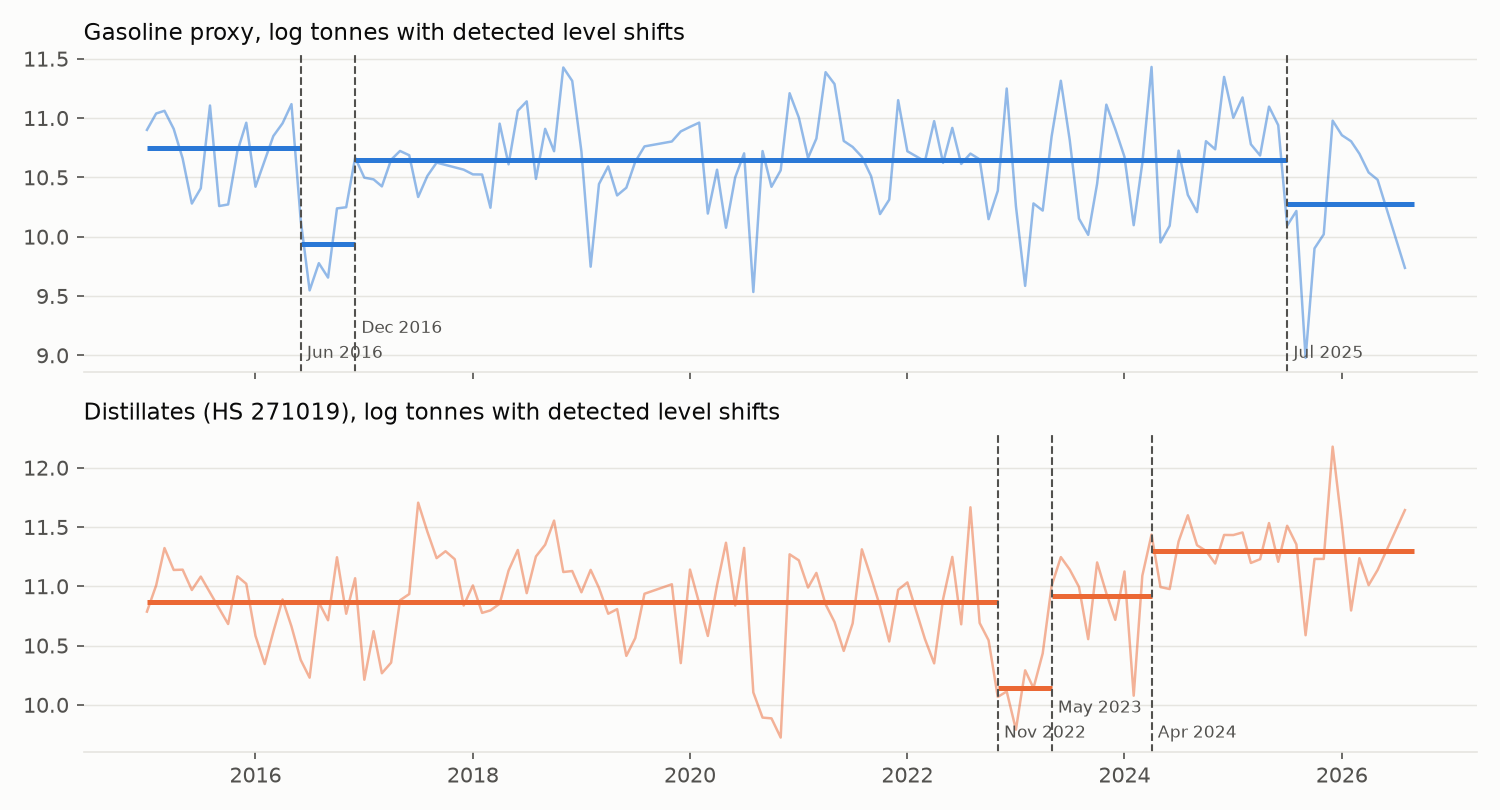
\includegraphics[width=\columnwidth]{fig05_kyrgyz_structural_breaks}
\caption{PELT level shifts in Kyrgyz log mass. Breaks describe shifts and do not prove causes.}
\label{fig:breaks}
\end{figure}

\subsection{Supplier Structure}
Partner rows with mass cover at least 90\% of import value in 99.4\% of 6,505 series-months. Kyrgyz gasoline has a median $\mathrm{HHI}^{12}$ of 0.89 (Fig.~\ref{fig:hhi}), so it varies little, which is a direct difficulty for H4. Net import dependency in 2024 was 0.77 for gasoline and 0.86 for diesel. Partner seems to mean origin or seller, not corridor, since Rwanda's and Zambia's leading partner is the UAE; this is an inference, so shared-supplier features may not measure shared route risk.

\begin{figure}[t]
\centering
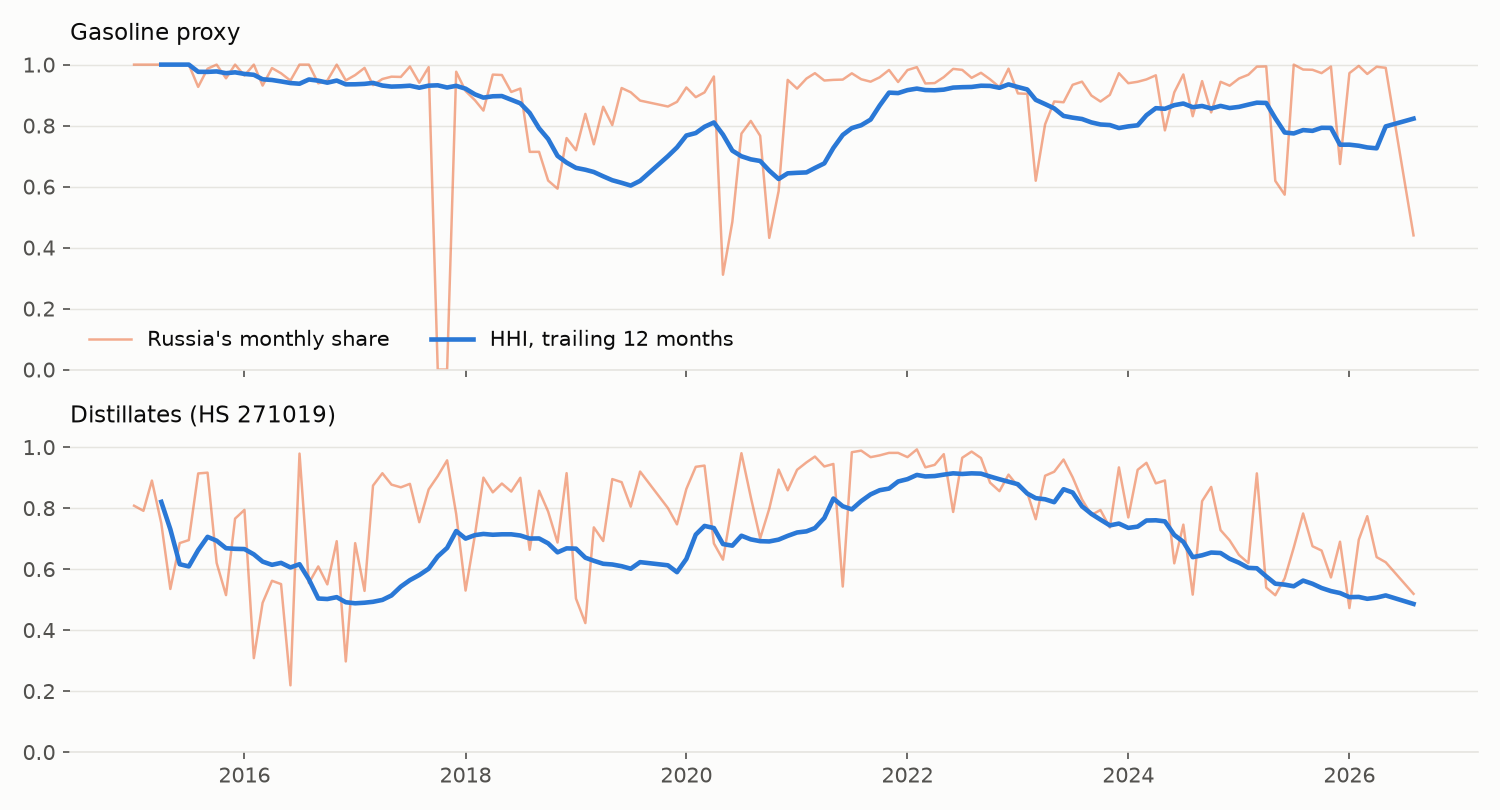
\includegraphics[width=\columnwidth]{fig08_kyrgyz_supplier_concentration}
\caption{Kyrgyz supplier concentration and Russia's monthly share.}
\label{fig:hhi}
\end{figure}

\subsection{External Indicators}\label{sec:external}
Spearman correlations on year-on-year log changes at leads of 0, 1, 3 and 6 months are weak. With Benjamini--Hochberg correction \cite{benjamini1995}, 155 of 862 tests pass across the panel, although overlapping windows make $p$-values too small and signs vary. For Kyrgyzstan, 0 of 40 pass. Weak linear correlation does not rule out a role during shocks, so the indicators are kept for ablation with modest expectations.

\subsection{Shortfall Labels}
On clean data, rule \eqref{eq:shortfall} gives 11 gasoline and 7 distillate episodes among 112 evaluable months, against 11 and 8 on the uncleaned data used in the proposal. Dates move, and September 2025 onward lies in the provisional period.

\subsection{Decision}
The data support a \textit{conditional go}. Before any model runs, the study must (1) have the cleaning and tier rules reviewed and frozen; (2) treat 2025--2026 as provisional and evaluate on data as first released; (3) take a second Comtrade snapshot, so revisions can be measured; (4) lag every feature to its release date; and (5) build a sourced event list before using shortfall labels.

\section{Proposed System Architecture}\label{sec:arch}

\subsection{End-to-End Architecture}
The artefact, the Fuel Import Risk Monitor, answers the research questions in a usable form (Fig.~\ref{fig:arch}). It composes existing components and introduces no new network type.

\begin{figure}[t]
\centering
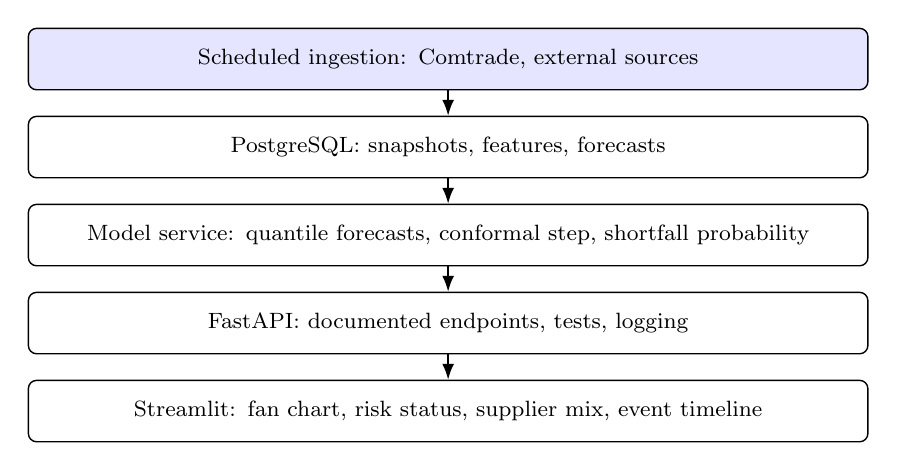
\begin{tikzpicture}[
  layer/.style={draw, rounded corners=3pt, align=center, font=\footnotesize, minimum height=0.78cm, text width=0.86\columnwidth, line width=0.5pt},
  arrow/.style={-{Latex[length=2mm]}, line width=0.6pt},
  node distance=0.32cm]
\node[layer, fill=blue!10] (a) {Scheduled ingestion: Comtrade, external sources};
\node[layer, below=of a] (b) {PostgreSQL: snapshots, features, forecasts};
\node[layer, below=of b] (c) {Model service: quantile forecasts, conformal step, shortfall probability};
\node[layer, below=of c] (d) {FastAPI: documented endpoints, tests, logging};
\node[layer, below=of d] (e) {Streamlit: fan chart, risk status, supplier mix, event timeline};
\foreach \x/\y in {a/b,b/c,c/d,d/e} \draw[arrow] (\x) -- (\y);
\end{tikzpicture}
\caption{Fuel Import Risk Monitor. The ingestion and database layers exist in the data pipeline; the others are planned.}
\label{fig:arch}
\end{figure}

\subsection{Data Engineering Layer}
This layer already exists. It stores every raw response with a retrieval date and hash, resumes from checkpoints, and writes versioned datasets. Twenty-four automated tests pass, and all 878 stored responses match their download hashes.

\subsection{Forecasting Layer}
The layer produces quantiles per series and horizon. Models are versioned, and each forecast is stored with its origin date, so past performance can be shown honestly.

\subsection{Calibration and Risk Layer}
A conformal step on a chronologically later window adjusts intervals, and \eqref{eq:risk} gives shortfall probability from the forecast distribution.

\subsection{Decision-Support Prototype}
A Streamlit client will show a fan chart, risk status, supplier mix and a documented event timeline, with Docker Compose for reproducible deployment. Any displayed number will come from actual model output. Because of publication lag, the monitor gives early warning, not a live feed.

\section{Experimental Design}\label{sec:exp}

\subsection{Experimental Objectives}
The experiments answer RQ1--RQ4 through controlled comparisons: (i) does a learned model beat simple baselines; (ii) does pooling help; (iii) does Deep Learning add value, and when; (iv) does supplier and shock information help; and (v) are probabilities calibrated and useful. Null results are reported with equal prominence. Table~\ref{tab:hyp} specifies variables for each hypothesis.

\begin{table*}[t]
\centering
\caption{Hypotheses with independent variables, dependent variables, comparison and metric.}
\label{tab:hyp}
\small
\begin{tabularx}{\textwidth}{@{}c X X X X@{}}
\toprule
H & Independent variable & Dependent variable & Comparison / baseline & Metric\\
\midrule
H1 & Global vs.\ local training & Kyrgyz forecast error, $h=3$ & Best local model & MASE, HLN test\\
H2 & Neural vs.\ boosted model & Error, normal and shock windows & LightGBM & MASE, pinball, stratified\\
H3 & Presence of supplier and shock features & Quantile error, high-dependence series & Own-history model & Pinball loss\\
H4 & Forecast probability vs.\ HHI ranking & Shortfall detection & HHI screening & PR-AUC, recall at alert budget\\
\bottomrule
\end{tabularx}
\end{table*}

\subsection{Baseline Experiments}
All models in Table~\ref{tab:models} use the same origins and horizons. Tuning budgets are matched to avoid advantaging complex models, and results are reported per horizon.

\subsection{As-of Replay}
At each origin only data released by that date are visible. For observations with $r_{it}$ unavailable, the reporter's median lag is used and marked. With a median Kyrgyz lag of 72 days in the pilot, $h=3$ from the last observed month corresponds roughly to the next month in real time.

\subsection{Shock Windows}
Results are stratified across the documented Russian restrictions and the 2026 Kyrgyz crisis \cite{gta2023,enerdata2024,gta2025,kwan2026}. Because data for June and July 2026 are absent for Kyrgyzstan, that crisis has thin coverage, and claims from a single event are avoided.

\subsection{Ablation Study}\label{sec:ablation}
The ablation design isolates the marginal value of each information source (Table~\ref{tab:ablation}). All arms use the same model family and tuning budget.

\begin{table}[t]
\centering
\caption{Ablation design.}
\label{tab:ablation}
\small
\begin{tabularx}{\columnwidth}{@{}c X L{2.5cm}@{}}
\toprule
ID & Removed or changed & Question\\
\midrule
A1 & Global replaced by local & RQ1, pooling\\
A2 & Strict importers only & RQ1, dissimilar panel\\
A3 & No supplier features & RQ3\\
A4 & No shock calendar & RQ3\\
A5 & No Brent, GPR, FX or CPI & RQ3, global conditions\\
A6 & No lagged unit value & RQ3, RQ4\\
A7 & Training stops before 2022 & Structural breaks\\
A8 & No conformal step & RQ4, calibration\\
A9 & Graph attention layer added & Graph vs.\ features\\
\bottomrule
\end{tabularx}
\end{table}

\subsection{Uncertainty Evaluation}
Empirical coverage at nominal 80\% and 95\%, mean interval width and pinball loss are compared with and without conformal calibration, on later test periods so that distribution shift is visible. Reporting both coverage and width prevents a trivial wide interval from scoring well.

\subsection{Shortfall Experiments}
Shortfall probability is compared with HHI ranking using PR-AUC, recall at a fixed alert budget and lead time, on pooled panel events. If labels prove too weak, classification is dropped and exceedance probabilities are reported alone.

\subsection{Robustness and Sensitivity}
Checks cover shortfall thresholds of 0.70, 0.75 and 0.80; baseline windows of two and three years; lag assumptions; exclusion of COVID-19 months; exclusion of 2015--2017 for Kyrgyzstan; at least five seeds; a real-time version of the cleaning rules; and Bai--Perron break tests \cite{bai2003}.

\subsection{Statistical Comparison}
Differences are assessed with the Harvey--Leybourne--Newbold corrected Diebold--Mariano test \cite{diebold1995,harvey1997}, with Holm correction and moving-block bootstrap intervals. Pairwise tests have low power on short test sets, so effect sizes are always reported, and statistical significance is distinguished from practical significance.

\section{Expected Results and Discussion Framework}\label{sec:expected}
No final results exist at this stage. This section states what types of result the study is expected to produce and how they will be interpreted, including outcomes that contradict the hypotheses.

\subsection{Pilot Evidence}
A small, deliberately untuned pilot tested whether the design runs. It used the earlier 43-series panel with World-row totals, without as-of replay, with test targets from September 2024 to August 2026 (Table~\ref{tab:pilot}). It establishes no ranking of models: about 22 Kyrgyz test months are too few, and no significance test was run. Next-three-month gasoline WAPE fell from about 28\% for the 12-month mean to about 21\% with local LightGBM, so signal exists. For August 2026, the median forecast was 38.1~kt with a lower bound of 20.5~kt, and the actual was 16.9~kt, so autoregressive features alone did not anticipate the shock.

\begin{table}[t]
\centering
\caption{Untuned pilot: Kyrgyz gasoline WAPE (\%). Lower is better; results are indicative only.}
\label{tab:pilot}
\small
\begin{tabular}{@{}lccc@{}}
\toprule
Model & $h=1$ & $h=3$ & Next 3 months\\
\midrule
Seasonal naive & 49.6 & 49.6 & 29.2\\
12-month mean & 38.9 & 39.5 & 28.4\\
LightGBM, local & 30.4 & 32.0 & 20.7\\
LightGBM, global & 30.6 & 34.8 & 23.6\\
GRU, global & 33.5 & 42.9 & 28.5\\
\bottomrule
\end{tabular}
\end{table}

\subsection{Expected Forecasting Results}
Error is expected to increase with horizon. Whether neural models match LightGBM will be judged by effect size and interval, and if differences are within noise, the conclusion will be that no advantage was demonstrated on these data.

\subsection{Expected Value of Pooling}
Weak co-movement suggests pooling may help through shared dynamics rather than shared shocks. A finding that pooling does not help Kyrgyzstan would be a legitimate result for H1, and the pilot does not yet support H1 for gasoline.

\subsection{Expected Value of Supplier Information}
Where HHI is near its ceiling, it has little room to discriminate between safe and risky months, so supplier share changes may matter more than the index. Kwon and Jeong's weak result for concentration \cite{kwon2026} may or may not hold where one supplier dominates.

\subsection{Expected Benefits of Calibration}
Conformal calibration is expected to bring coverage closer to nominal levels, at the cost of wider intervals. Its usefulness depends on stability, and shocks may break it.

\subsection{Expected Shortfall Results}
Rare events are expected, so PR-AUC and calibration will be more informative than accuracy. Results will carry confidence intervals, and models cannot be expected to foresee a policy decision. What they may show is how quickly risk rises after early signals.

\subsection{Practical Implications}
If supported, the results could inform stock planning against the 2.5-month target and supplier diversification for planners and fuel traders. These implications are conditional on empirical findings, and the system remains a research prototype.

\section{Limitations, Ethics and Research Risks}\label{sec:limits}

\subsection{Customs Data Limitations}
Customs records are not consumption, and stocks, local refining and informal trade lie outside the monthly data. Six reporters appear to file fuels under another HS line. Monthly and annual Comtrade disagree for some reporter-years, which stay flagged.

\subsection{Provisional and Revised Data}
This is the most serious limitation. Recent records are provisional, and training on later-revised values would give a forecaster information it never had. First-release evaluation and repeat snapshots address it, but the true size of the 2025--2026 shock stays uncertain until the 2025 balance appears.

\subsection{Product Definition Uncertainty}
HS~2710.19 mixes products. Conclusions on distillates cannot be read as conclusions on diesel, and gasoline remains the cleanest target.

\subsection{Rare Events}
Documented shocks are few, and the newest are the least certain. Causal interpretation is unsafe, and single events will not support general claims.

\subsection{Panel Heterogeneity}
The panel mixes exporters, transit markets, microstates and low-income importers. Importer types were set by hand and must be verified against named sources, or the strict-importer ablation will be dropped.

\subsection{Modelling Assumptions}
Assumptions include a useful stability within training windows, adequacy of the shortfall baseline, and approximate exchangeability for conformal coverage. Overfitting risk grows with model capacity relative to the number of independent observations. The cleaning thresholds are judgment calls awaiting supervisor review.

\subsection{Ethical and Academic Considerations}
All data are public, aggregate and non-personal. API keys are kept in the environment and out of the repository. The work is supply-chain decision support and gives no guidance for evading trade restrictions. Faculty rules limit combined plagiarism and AI-generated content to 30\% and require AI prompt records, so AI assistance in this project is disclosed, and every result must be explainable by the author at the defence.

\section{Conclusion and Future Work}\label{sec:conclusion}

\subsection{Summary of Proposed Research}
The proposal formulates monthly fuel-import and shortfall-risk forecasting as a probabilistic problem for landlocked economies, with Kyrgyzstan as the case. A completed data stage shows that the target can be validated, that a small global panel is feasible, and that the newest records must be handled as first releases. A rolling-origin protocol, a staged model progression, an ablation design and calibration-focused evaluation will establish whether added complexity yields measurable benefit.

\subsection{Expected Scientific Contribution}
The expected scientific contribution is a tested benchmark under real publication lag, including evidence on when pooling and supplier information help and when they do not. No novel architecture is claimed.

\subsection{Expected Practical Contribution}
The expected practical contribution is a reproducible pipeline and a public-data monitor for research and planning.

\subsection{Future Research}
Possible extensions include official monthly fuel tonnage from NSC or customs, eight- or ten-digit customs data that separate diesel from gasoline, production and consumption data that extend dependency beyond Kyrgyzstan, repeated snapshots that model revisions directly, and more shock events as data accumulate.

\bibliographystyle{IEEEtran}
\bibliography{references}

\end{document}
